
% !TEX root = ../paper.tex

\section{Distributional Reduction}\label{sec:DDR}


The previous interpretation is significant because it allows for two generalizations. Firstly, beyond solely determining the positions $\vz_i$ of Diracs (as in classical DR) we can now optimize \emph{the mass} of the distribution $\mu_Z$. This is interpreted as finding the relative importance of each point in the embedding $\mZ$. More importantly, due to the flexibility of GW, we can also seek a distribution in the embedding with a smaller number of points $n < N$. This will result in both reducing the dimension \emph{and} clustering the points in the embedding space through the optimal coupling. Informally, our \emph{Distributional Reduction} (DistR) framework aims at solving $\min_{\mu_Z \in \gP_n(\R^d)} \GW(\frac{1}{n} \sum_{i=1}^{N} \delta_{\vx_i}, \mu_Z)$.

% In light of the presented characterization of dimensionality reduction as a GW projection of a discrete distribution, we present the  (Dist-DR) problem.

\subsection{Distributional Reduction Problem}\label{sec:DDR_ob}

Precisely, the optimization problem that we tackle in this paper can be formulated as follows
\begin{align}\tag{DistR}\label{eq:Dist-DR}
	\min_{\begin{smallmatrix} \mZ \in \R^{n \times d} \\ \vh_Z \in \Sigma_n \end{smallmatrix}} \GW_L (\simiX(\mX), \simiZ(\mZ), \vh_X, \vh_Z)
\end{align}
%where $\mZ \in \R^{n \times d}$, $\vh_Z \in \R^n$ .
This problem comes down to learning the closest graph $(\mC_Z(\mZ), \vh_Z)$ parametrized by $\mZ$ from $(\mC_X(\mX), \vh_X)$ in the GW sense. When $n < N$, the embeddings $(\vz_1, \cdots, \vz_n)$ then act as \emph{low-dimensional prototypical examples} of input samples, whose learned relative importance $\vh_Z$ accommodates clusters of varying proportions in the input data $\mX$ (see \Cref{fig:general_idea}). We refer to them as \emph{prototypes}. The weight vector $\vh_X$ is typically assumed to be uniform, that is $\vh_X=\frac{1}{N} \one_N$, in the absence of prior knowledge. As discussed in \Cref{sec:DR_as_OT}, traditional DR amounts to setting $n = N, \vh_Z = \frac{1}{N} \one_N$.

\paragraph{Clustering with DistR.} One notable aspect of our model is its
capability to simultaneously perform dimensionality reduction and clustering.
Indeed, the optimal coupling $\mT \in [0, 1]^{N \times n}$ of problem
\cref{eq:Dist-DR} is, by construction, a soft-assignment matrix from the input
data to the embeddings. It allows each point $\vx_i$ to be linked to one or more
prototypes $\vz_j$ (clusters). In \Cref{sec:clustering_properties} we explore
conditions where these soft assignments transform into hard ones, such that each
point is therefore linked to a unique prototype/cluster.

% \begin{figure*}[t!]
% 	\begin{center}
% 		\centerline{\includegraphics[height=3.3cm]{figures/grids/PCA_embeddings.pdf}
% 			\includegraphics[height=3.3cm]{figures/grids/srGWprojections_largegrid_PCA_px16_cut.pdf}
% 			\includegraphics[height=3.3cm]{figures/grids/srGWprojections_largegrid_PCA_px32_cut.pdf}
% 			\includegraphics[height=3.3cm]{figures/grids/srGWprojections_largegrid_PCA_px64_cut.pdf}
% 			\includegraphics[height=3.3cm]{figures/grids/srGWprojections_largegrid_PCA_px96_cut.pdf}
% 		}
% 		%\centerline{\includegraphics[height=3cm]{figures/grids/kernelPCA_embeddings.pdf}
% 		%	\includegraphics[height=3cm]{figures/grids/srGWprojections_largegrid_kernelPCA_px16_cut.pdf}
% 		%	\includegraphics[height=3cm]{figures/grids/srGWprojections_largegrid_kernelPCA_px32_cut.pdf}
% 		%	\includegraphics[height=3cm]{figures/grids/srGWprojections_largegrid_kernelPCA_px64_cut.pdf}
% 		%	\includegraphics[height=3cm]{figures/grids/srGWprojections_largegrid_kernelPCA_px96_cut.pdf}}
% 		\caption{GW projections of a single-cell genomics dataset \citep{chen2019high} on regular grids with increasing resolutions, respectively encoded as $C_X(\mX) = \mX \mX^\top$ and $C_Z(\mZ) = \mZ \mZ^\top$. Pixels on cropped grids are colored by interpolating samples' colors according to the transport plan and their intensity is proportional to their mass.}
% 		\label{fig:visu_fixedsupport}
% 	\end{center}
% 	\vspace{-0.8cm}
% \end{figure*}


\paragraph{A semi-relaxed objective.} For a given embedding $\mZ$ and $L=L_2$, it is known that minimizing in $\vh_{Z}$ the DistR objective is \emph{equivalent} to a problem that is computationally simpler than the usual GW one, namely the semi-relaxed GW divergence $\srGW_L$ \citep{vincent2021semi}:
\begin{equation*}\tag{srGW} \label{eq:srGW}
	\min_{\mT \in \gU_n(\vh_X)} E_L(\simiX(\mX), \simiZ(\mZ), \mT) \:,
\end{equation*}
where $\gU_n(\vh_X) := \left\{ \mT \in \R_{+}^{N \times n}: \mT \one_n = \vh_X\right\}$. To efficiently address \cref{eq:Dist-DR}, we first observe that this equivalence holds for any inner divergence $L$ with a straightforward adaptation of the proof by \citet{vincent2021semi}.
%We complete our analysis with the following result.
%\begin{proposition}\label{prop:srgw_divergence}
%	For any divergence $L$, \ref{eq:srGW} vanishes iif there exists $\vh_Z \in \Sigma_n$  such that $(\mC_X(\mX), \vh_X)$ and $(\mC_Z(\mX), \vh_Z)$ are weakly isomorphic. \tv{vraiment besoin d'une prop ? comme ona pas def weakly isom, juste un commentaire ?}
%\end{proposition}
Additionally, we prove that $\srGW_L$ remains a divergence as soon as $L$ is itself a divergence. Consequently, $\srGW_L$ vanishes iff both measures are isomorphic in a weak sense \citep{chowdhury2019gromov}. We emphasize that taking a proper divergence $L$ is important (and basic assumptions on $\mX$), as it avoids some trivial solutions as detailed in Appendix \ref{sec:srGW_divergence}.

%The latter notion may introduce trivial solutions into our \ref{eq:Dist-DR} problem which can be avoided with basic assumptions over $\mu_X$, always verified in our experiments, that we discuss .   

%We assume without loss of generality 
%Assuming that $\mX$ does not admit duplicate samples, otherwise one could
%aggregate their total mass, most applications $C_X$ result in a graph
%$(\mC_X(\mX), \vh_X)$ which is irreducible w.r.t the notion of weak
%isomorphism. As such, proposition \ref{prop:srgw_divergence} implies that
%setting any $n < N$ in \ref{eq:Dist-DR} guarantees clustering of samples in
%$\mC_X(\mX)$. \tv{comprends pas cette derniere phrase + pourquoi en as t'on
%besoin ?}



Interestingly, srGW projections, \textit{i.e.} optimizing only the weights $\vh_Z$ over simple fixed supports $\mZ$, have already remarkable representational capability. We illustrate this in \Cref{fig:visu_fixedsupport}, by considering projections of a real-world dataset over 2D grids of increasing resolutions. Setting $\mC_X(\mX) = \mX \mX^\top$ and $\mC_Z(\mX) = \mZ \mZ^\top$, we can see that those projections recover faithful coarsened representations of the embeddings learned using PCA. DistR aims to exploit the full potential of this divergence by learning a few optimal prototypes that best represent the dataset.

%We can see that  thus providing a new alternative to standard \ref{eq:DR_criterion} by optimizing the weights $\vh_Z$ instead of the locations $\delta_{\vz_i}$.



\subsection{Clustering Properties \label{sec:clustering_properties}}

In addition to the connections established between DistR and DR methods in \Cref{sec:DR_as_OT}, we elaborate now on the links between DistR and clustering methods.% in this section. 

In what follows, we call a coupling $\mT \in [0,1]^{N \times n}$ with a single non-null element per row a \emph{membership matrix}. When the coupling is a membership matrix each data point is associated with a single prototype thus achieving a hard clustering of the input samples.

% Though the link between \ref{eq:Dist-DR} and existing DR methods is made explicit by \Cref{theo:main_theo}, relating \ref{eq:Dist-DR} to known clustering algorithms is not straightforward \tv{je vais reformuler de manire positive: en plus des liens avec le DR on peut faire des liens avec le clustering}. 


% Recall that \ref{eq:Dist-DR} focuses on finding the embedding distribution $\mu_Z =\sum_{i=1}^n [\vh_Z]_i \delta_{\vz_i} \in \gP_n(\R^d)$ while imposing a specific geometry, induced by $C_Z$, over the embeddings. 

% We emphasize its differences with the problem known as \emph{srGW barycenter} \citep{vincent2021semi}, that seeks for a closest target graph $(\overline{\mC}, \overline{\vh})$ from $(\mC_X, \vh_X)$ without any assumption, or control, over the support of the target distribution: 

%the \emph{srGW barycenter} \citep{vincent2021semi}, %is however strongly connected to \ref{eq:Dist-DR}.
%and not only a target graph $(\overline{\mC}, \vh_Z)$. \tv{a reformuler}
%  whose support would be let implicit,	
% The latter problem, known as the \emph{srGW barycenter} \citep{vincent2021semi}, is however strongly connected to \ref{eq:Dist-DR}.
We will see that a link can be drawn with kernel K-means using the analogy of \emph{GW barycenters}. More precisely the \emph{srGW barycenter} \citep{vincent2021semi} seeks for a closest target graph $(\overline{\mC}, \overline{\vh})$ from $(\mC_X, \vh_X)$ by solving
\begin{equation}\tag{srGWB}\label{eq:srGBW}
	\min_{\overline{\mC} \in \R^{n \times n}} \min_{\mT \in \mathcal{U}_n(\vh_X)} E_L(\simiX(\mX), \overline{\mC}, \mT) \:.
\end{equation} 
We emphasize that the only (important) difference between \cref{eq:srGBW} and
\cref{eq:Dist-DR} is that there is no constraint imposed on $\overline{\mC}$ in
srGWB. In contrast, \cref{eq:Dist-DR} looks for minimizing over $\overline{\mC}
\in \{\simiZ(\mZ): \mZ \in \R^{N \times d}\}$. For instance, choosing $\simiZ(\mZ) = \mZ \mZ^\top$ in \cref{eq:Dist-DR} is
equivalent to enforcing $\operatorname{rank}(\overline{\mC}) \leq d$ in
\cref{eq:srGBW}.
\begin{figure*}[t!]
	\begin{center}
		\centerline{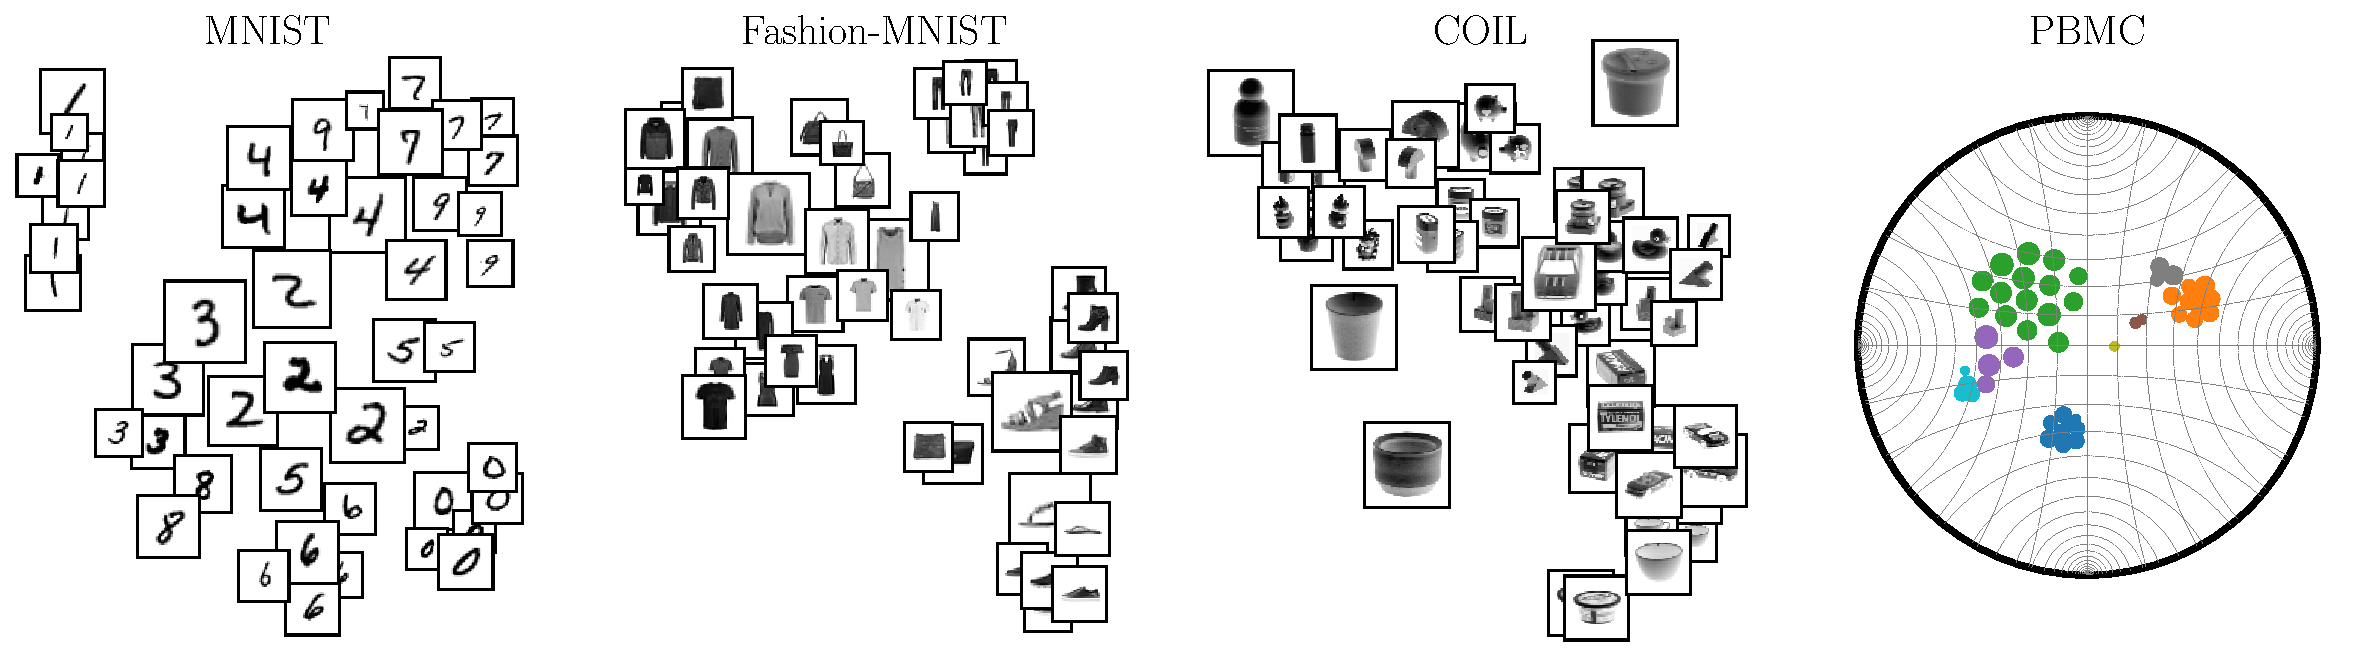
\includegraphics[width=\columnwidth]{figures/DistR/DistDR_embed.pdf}}
		\caption{Examples of 2-dimensional embeddings produced by DistR using the SEA similarity for $\simiX$ 
		and the Student's kernel for $\simiZ$. The latter computed in $\R^2$ for the first three datasets and the Poincaré ball for the last one.
		Displayed images are medoids for each cluster \ie $\argmax_i [\mC_X(\mX)\mT_{:,k}]_i$ for cluster $k$. The area of image $k$ is proportional to $[\vh_Z]_k$.
		}
		\label{fig:visu_gwdr}
	\end{center}
	\vspace{-0.8cm}
\end{figure*}

We establish below that srGWB is of particular interest for clustering. The motivation for this arises from the findings of \citet{chen2023gromov}, which demonstrate that when $\simiX(\mX)$ is positive semi-definite and $\mT$ is \emph{constrained} to belong to the set of membership matrices (as opposed to couplings in $\gU_n(\vh)$), \cref{eq:srGBW} is equivalent to a kernel K-means whose samples are weighted by $\vh_X$ \citep{dhillon2004kernel, dhillon2007weighted}. These additional constraints are in fact unnecessary since we show below that the original srGWB problem admits membership matrices as the optimal coupling for a broader class of $\simiX(\mX)$ input matrices (see proofs in appendix \ref{sec:srGW_concavity}).%by demonstrating that the constraint on $\mT$ to be a membership matrix is, in fact, unnecessary. We show below that the original srGWB problem admits  membership matrices as optimal coupling for a broader class of input matrices $\simiX(\mX)$ (see proofs in Appendix \ref{sec:srGW_concavity}).
% seminal result in this direction from  considered $\mC_X(\mX)$ PSD and the combinatorial (Monge) counterpart of the \ref{eq:srGBW} problem. 
\begin{restatable}{theorem}{baryconcavity}
	\label{theo:srgw_bary_concavity}
	Let $\vh_X \in \Sigma_N$ and $L=L_2$. Suppose that for any $\mX \in \R^{N \times p}$ the matrix $\simiX(\mX)$ is CPD or CND. Then the problem \cref{eq:srGBW} admits a membership matrix as optimal coupling, \ie, there is a minimizer of $\mT \in \mathcal{U}_n(\vh_X) \to \min_{\overline{\mC} \in \R^{n \times n}}  E_L(\simiX(\mX), \overline{\mC}, \mT)$ with only one non-zero value per row.
	% optimal transports. %extremities of $\mathcal{U}_n(\vh)$ as optimum.
\end{restatable}
% The sufficient condition in Theorem \ref{theo:srgw_bary_concavity} is satisfied for existing DR methods (\Cref{sec:dr_methods}), \emph{e.g} when $\mC_X$ outputs a PSD, NSD or a squared Euclidean distance matrix . 
% Notice that we also establish a corollary of \Cref{theo:srgw_bary_concavity} providing an analog result when masses on $\overline{\mC}$ are not optimized. 
%These relations and \Cref{theo:srgw_bary_concavity} further legitimize the use of GW projections for clustering and allow us to expect OT plans of \ref{eq:Dist-DR} to be close to providing a hard-clustering of $\mX$. \tv{a reformuler}
\Cref{theo:srgw_bary_concavity} and relations proven in \citet{chen2023gromov} provide that  \cref{eq:srGBW} is equivalent to the aforementioned kernel K-means when $\mC_X(\mX)$ is positive semi-definite. Moreover, as the (hard) clustering property holds for more generic types of matrices, namely CPD and CND, srGWB stands out as a fully-fledged clustering method.
Although these results do not apply directly to DistR, we argue that they further legitimize the use of GW projections for clustering. Interestingly, we also observe in practice that the couplings obtained by DistR are always membership matrices, regardless of $\simiZ$. Further research will be carried out to better understand this phenomenon. 
%and allow us to believe that the OT of DistR are close to providing hard clustering. We point out that it was always the case in our experiments.
%When $\vh$ is uniform, these extremities are membership matrices up to a factor $\frac{1}{N}$ \cite[Theorem 1]{cao2022centrosymmetric}. 
%Interestingly, 

%\hva{à retravailler/incorporer} Following \citep{vayer2018optimal}
% (equation 6) , we can also see that $g$ is convex whenever the GW problem from a graph to itself is concave. Hence Proposition 2 from \citep{redko2020co} also extends our analysis %, we can conclude that our sufficient condition is also satisfied when $\mC_X$ is a  to squared Euclidean distance matrices. % \hva{or a PSD matrix} as often in DR \hva{(see \cref{sec:DR_methods})}.

\subsection{Computation}\label{sec:computation_GW}

DistR is a non-convex problem that we propose to tackle using a Block Coordinate Descent algorithm (BCD, \citealt{tseng2001convergence}) guaranteed to converge to local optimum \citep{grippo2000convergence, Lyu2023bmm}. The BCD alternates between the two following steps. First, we optimize in $\mZ$ for a fixed transport plan using gradient descent with adaptive learning rates \citep{kingma2014adam}. Then we solve for a srGW problem given $\mZ$. To this end, we benchmarked both the Conditional Gradient and Mirror Descent algorithms proposed by \citet{vincent2021semi}, extended to support losses $L_2$ and $L_{\KL}$.

Following Proposition 1 in \citep{peyre2016gromov}, a vanilla implementation leads to $\mathcal{O}(n N^2 + n^2N)$ operations to compute the loss or its gradient. In many DR methods, $\mC_X(\mX)$ or $\mC_Z(\mZ)$, or their transformations within the loss $L$, admit explicit low-rank factorizations. Including \emph{e.g.} matrices involved in spectral methods and other similarity matrices derived from squared Euclidean distance matrices \citep{scetbon2022linear}. In these settings, we exploit these factorizations to reduce the computational complexity of our solvers down to $\mathcal{O}(Nn(p + d) + (N + m)pd + n^2)$ when $L=L_2$, and $O(Nnd + n^2d)$ when $L = L_{\KL}$. We refer the reader interested in these algorithmic details to Appendix \ref{sec:algorithms}.
%By leveraging the low-rank natures of structures $\mC_X(\mX)$ and $\mC_Z(\mZ)$ encountered in many DR methods, or of their transformations within $L$, the computational complexity can be reduced up to $\mathcal{O}(Nn(p + d) + (N + m)pd)$ \tv{a discuter plus : c'dst linear ! + quelle genre de low rank + citer cutu}. \citep{scetbon2022linear} - We refer the reader interested in these algorithmic details to Appendix X \tv{attention}.
%The complexity of each update is majorized by the computation of the objective \cref{eq:gw_pb} which scales in $\mathcal{O}(nN^2 + n^2N)$.

% \textbf{Computation.}	We adopt a block coordinate strategy, iteratively solving the OT and embedding subproblems.
% % \begin{align}
	% %     \mZ \xleftarrow[]{} \argmin_{\mZ \in \R^{n \times d}} \: \sum_{k \in \integ{K}} \mathrm{srGW}_L(\mC_k, \vh, \mC_Z) \:.
	% % \end{align}
% Motivated by the
% envelope theorem \citep{carter2001foundations}\cvc{BCD you dont need to mention this}, we do not backpropagate the gradient through the iterative computation of the GW plan. The complexity of each update is majorized by the computation of the objective \cref{eq:gw_pb} which scales in $\mathcal{O}(nN^2 + n^2N)$. Note that relaxing the marginal constraint in srGW makes the rows of the OT plan independent thus leading to a significant reduction of the computational cost compared to regular GW \cvc{we dont care about that}. 
% \begin{algorithm}[h]
	% 	\caption{\textit{BCD for Joint Clustering and Dimensionality Reduction}}
	% 	\label{algo:BCD_partitioned_affinities}
	% 	\begin{algorithmic}[1]
		% 		\STATE {\bfseries Input: $\mC_X$} \\
		% 		\WHILE{not converged}
		% 		  \STATE $\mT \xleftarrow[]{} \argmin_{\mT \in \mathcal{U}_{\bm{h}, \overline{\bm{h}}}} \: \mathcal{E}(\mC_X, \mC_Z, \mT)$ 
		% 		  \\
		% 		  \STATE $\mZ \xleftarrow[]{} \argmin_{\mZ \in \R^{n \times d}} \: \mathcal{E}(\mC_X, \mC_Z, \mT)$ 
		% 		  \\
		% 		\ENDWHILE
		% 		\STATE {\bfseries Output: $\mZ$}
		% 	\end{algorithmic}
	% \end{algorithm}

% \textbf{Related work multi-view.}
% In \citep{gong2022gromov}, an encoder neural network is learned for each view such that the GW barycenter of the input kernels matches the identity matrix. 

% Library \citep{perry2021mvlearn}

% Multi-view MDS \citep{trendafilov2010stepwise}

% \textbf{Multi-Scale Dimensionality Reduction.}
% A long-standing problem in DR is to construct embeddings that can faithfully account for both close and large-scale dependencies as most popular approaches including SNE-like algorithms (\textit{e.g.}\ UMAP \citep{mcinnes2018umap} or t-SNE \citep{van2008visualizing}) usually fail in this task. % (see \emph{e.g} \cref{fig:multi_scale}).
% To remedy this, two main approaches are considered in practice. The first handles the large-scale structure at initialization and then runs a SNE-like method on top of it with relatively small perplexity\footnote{SNE-like methods adaptively set a kernel bandwidth for each point based on the 'perplexity' hyperparameter that can be intuitively interpreted as the number of effective neighbors of each point.} 
% % to capture fine-grained structure 
% \citep{van2023snekhorn, kobak2021initialization} while the second 
% % This assumes that the initial structure will be preserved in the course of the embedding optimization, which is unfortunately often not the case 
% consists of averaging multiple similarity matrices associated with various perplexities \citep{lee2015multi}.
% Both approaches generally lead to unsatisfactory results as shown in \cref{fig:multi_scale}.
% % The first is to handle the large-scale structure at initialization and then run a SNE-like method on top of it with relatively small perplexity to capture fine-grained structure \citep{van2023snekhorn}.
% % This assumes that the initial structure will be preserved in the course of the embedding optimization, which is unfortunately often not the case \citep{kobak2021initialization}. The second approaches boils down to averaging multiple similarity matrices associated with various scales (or perplexities) \citep{lee2015multi} but it generally leads to unsatisfactory results as shown in \cref{fig:multi_scale}. 
% Based on this observation, we propose a new approach that leverages our model. %the \cref{eq:GW_DR_pb} model. 
% We first compute prototypes $\mZ \in \R^{n \times d}$ by solving \cref{eq:GW_DR_pb} using a large scale affinity $\mC^{L}_X$
% and then position embeddings $\mY \in \R^{N \times d}$ using a small scale affinity $\mC^{\ell}_X$ under barycentric constraint given by the prototypes
% \begin{align}
	% \mY = \argmin_{\mY \in \R^{N \times d}} \mathrm{srGW}_L(\mC^{\ell}_X, \vh, \mC_Y) \quad \text{s.t.} \quad \diag(\vh) \mY \mT_Z = \mZ
	% \label{eq:multiscale_DR}
	% \end{align}
% where $\mT_Z$ is the OT plan associated with prototypes $\mZ$. 
% The above problem ensures that the embeddings' position is consistent with the prototypes computed using a larger scale of dependency.

\subsection{Related Work}\label{sec:related_work}

%The closest to our work is CO-Optimal Transport  in which the
% GW framework is extended to compute OT plans between both samples and features
% of two datasets of different sizes. 
The closest to our work is the CO-Optimal-Transport (COOT) clustering approach proposed in \citep{redko2020co} that estimates simultaneously a clustering of samples and features through the CO-Optimal Transport problem,
% \tv{pas sur d'avoir besoin de la formule ça prend de la place}
\begin{align}\tag{COOT}
	\label{eq:coot_pb}
	\min_{\substack{\mT_1 \in \gU(\vh_1, \overline{\vh}_1) \\ \mT_2 \in \gU(\vh_2, \overline{\vh}_2)}} \: \sum_{ijkl} (X_{ik} - Z_{jl})^2 [\mT_1]_{ij} [\mT_2]_{kl} \,,
\end{align}
where $\vh_1 \in \Sigma_N$, $\overline{\vh}_1 \in \Sigma_n$, $\vh_2 \in \Sigma_p$ and $\overline{\vh}_2 \in \Sigma_d$.
We emphasize that COOT-clustering, which consists in optimizing the COOT objective
above \emph{w.r.t.} $\mZ$, is a linear DR model as the reduction is done with the map $\mT_2$. In contrast, DistR
leverages the more expressive non-linear similarity functions of existing DR
methods. Other joint DR-clustering approaches, such as \citep{liu2022joint},
involve modeling latent variables by a mixture of distributions. In comparison,
our framework is more versatile, as it can easily adapt to any $(L, \mC_X,
\mC_Z)$ of existing DR methods (\Cref{sec:dr_methods}).
%\citep{collas2023entropic}